% !TEX root =single_chapter_ga.tex
\chapter{Genetic Algorithms}
\label{chap:ga}
\section{Introduction}
Numerical mathematics has been developing steadily over the last century and especially over the last 50 years when computers became readily available.  Like many other sciences numerical mathematics has been getting much inspiration from nature.  Advancements in our understanding of the brain, inspired numerical mathematicians to recreate some of the structures of this biological computer. These attempts resulted in Neural Networks which today have wide applications in many areas of science and engineering. Optimization algorithms, which are a sizeable subfield of numerical mathematics have also borrowed heavily from nature. Some examples are Ant Colony Optimization and Particle Swarm Optimization. The timeline in Figure \ref{fig:timeline} shows some of the milestones in optimization.

\begin{figure}
\begin{chronology}[5]{1965}{2000}{2.5ex}{\textwidth}
\event{1965}{Simplex optimization; Evolution strategies}
%\event{1966}{Evolutionary programming}
\event{1975}{Genetic Algorithms}
\event{1983}{Simulated Annealing}
\event{1992}{Ant Colony Optimization}
\event{1993}{multiobjective Genetic Algorithms}
\event{1995}{Particle Swarm Optimization \glsentryname{nfl} theorem}
\event{1997}{Differential Evolution}
\end{chronology}

\caption{Timeline of milestones in numerical optimization}
\label{fig:timeline}
\end{figure}

Biological evolution can be seen as an optimization algorithm that adjusts organisms to adapt perfectly to their environment.  The idea of an algorithm which imitates the principal of natural evolution was first introduced by \citet{Holland:1962:OLT:321127.321128}. Shortly after other groups independently started using similar approaches \citep[e.g.][]{Rechenberg1973}. The entire field of evolutionary algorithms has since split up into many subfields (e.g. genetic programming, evolutionary programming, evolution strategy, etc.). Out of these subfields, the \glspl{ga} are the most widely known and have been applied to many different problems. 

In general, optimization algorithms have two seemingly conflicting goals: exploiting good leads (optimum seeking) while still exploring the parameter space sufficiently. Simple algorithms like Hillclimbing (randomly selecting a point in the neighbourhood of the current point and then picking the more optimal point as the new basis) will exploit good leads but will neglect to explore the search space often leading to the convergence on local optima. Random searches, on the other hand, are excellent at exploring the search space but will fail to quickly converge on an optimal solution (and are not guaranteed to converge at all). Which algorithm to use, naturally depends on the type of parameter space. Spaces with independent variables can be solved relatively simply by employing optimum seeking methods. Random search algorithms are suited to parameter spaces with highly correlated variables. 
One should note that the better an algorithm is optimized for a specific search space the more poorly it performs on other problems. This constitutes the so called  \gls{nfl} , which also states that across the space of all problems, all algorithms perform equally well. \glspl{ga} seem to strike a balance between exploration and exploiting the current best solution. Consequently they can be applied to a wide range of different parameter spaces. In addition, they have many options and fine tuning parameters so that one can adjust them to individual problems. 

\section{Genetic Algorithms}
\glspl{ga} are a stochastic search technique that tries to find solutions in n-dimensional search spaces. In most optimization algorithm we have a function $f(\vec{x})=s$, where $\vec{x}$ is are the input parameters and $s$ is a solution scalar (sometimes referred to as figure-of-merit). The goal is to find the input parameters that optimize $s$ (finding a maximum or minimal value of $s$). In some optimization algorithms, however,  this function $f(\vec{x})$ does not immediatley produce a scalar solution $s$ but instead produces a solution vector $\vec{y}$ (e.g. curve fitting where input coefficients produce a number of output points). This gives two option, first we can find a function $g(\vec{y})=s$ that maps the solution to an optimizable scalar and proceed as above, or we can try to optimize the individual components of $\vec{y}$ simultatneously. The latter option is called multi-objective optimization and is a vast field of research, but outside the scope of this work. From now on we will consider that we have a function $f(\vec{x})=\vec{y}$ and a function $g(\vec{y})=s$. 

\glspl{ga} have terms for the described functions and parameters that borrow heavily from evolutionary science. The individual input parameters of $\vec{x}$ are often referred to as \glspl{gene}. The input vector $\vec{x}$ is called \gls{individual} or sometimes \gls{genome}. We refer to representation in parameter space as \gls{genotype} ($\vec{x}$) and the representation in solution space as  \gls{phenotype} ($\vec{y}$) of a solution. This is similar to biology where the input $\vec{x}$ can be thought of as the DNA sequence. The \gls{phenotype} in biology however does not resemble a vector (strictly speaking).  Mathematically speaking it is possible to have multiple \glspl{genotype} map to one \gls{phenotype}, however each \gls{genotype} only maps to one phenotype. 
One should also note that in many, if not most, optimization problems there exists no \gls{phenotype} as the function $f(\vec{x})$ maps directly to the optimizable scalar $s$. Finally, the function that results in the figure-of-merit ($f(\vec{x})=s$ or $g(\vec{y})=s$) is called the \gls{fitness} function which results in the \gls{fitness} $s$. 

In general, \glspl{ga} maintain a pool of \glspl{individual} called a population or generation. The general idea is that each new generation is created out the old generation. Owing to the special processes of the \gls{ga} each new generation will consist of \glspl{individual} that are on average closer to the optimal solution than the last generation. Following the notation of \citet{Michalewicz:1994:GAD:184675} we introduce the population $P(t)$ with the \glspl{individual}  $\{p_{1}^{t}, \dots, p_{n}^{t}\}$, where $t$ denotes the iteration (or generation number). Each individual $(p_{i}^t)$ is a data structure consisting of a vector $\vec{x}_i$ and its corresponding fitness scalar $s_i$.  When we speak of evaluating $p_{i}^{t}$ we mean that we use $g(f(\vec{x}_i))=s_i$ to determine the fitness. A new population (or generation) $P(t+1)$ is formed by choosing, in the \textit{select step}, the more fit individuals. Some or all of the new population undergo transformations in the \textit{recombine step}. These transformations are called genetic operators. We define unary transformations, which create new individuals by small changes in single individuals called \glspl{mutation}. Higher order transformations called \glspl{crossover} combine the traits of multiple individuals to form a next generation individual. 
After the new population has been created in the \textit{recombine step}, it is evaluated (perform the computation $g(f(\vec{x}_i))=s_i$) and the \textit{select step} begins anew. 

This procedure is repeated until some termination condition is reached (see Algorithm \ref{alg:evol_program}). One way is to wait until best individual in a generation or the whole generation has reached a certain threshold fitness.  Another way is to set a limit on the number of generations. 



\begin{pseudocode}{Genetic Algorithm}{ }
\label{alg:evol_program}
\PROCEDURE{Genetic Algorithm}{}
t \GETS 0 \\
\CALL{Initialize}{P(t)}\\
\CALL{Evaluate}{P(t)}\\
\WHILE (\textrm{\textbf{not} termination condition}) \DO
\BEGIN
t \gets t+1\\
P(t) \GETS \CALL{Select}{P(t-1)}\\
\CALL{Recombine}{P(t)}\\
\CALL{Evaluate}{P(t)}\\
\END
\ENDMAIN
\end{pseudocode}

%\renewcommand{\thepseudonum}{\roman{pseudonum}}
%\begin{pseudocode}{MergeSort}{n,X}
%\label{MergeSort}
%\COMMENT{Sort the array $X$ of length $n$}\\
%\IF n=2 \THEN
%\BEGIN
%\IF X[0]>X[1] \THEN
%\BEGIN
%T \GETS X[0]\\
%X[0]\GETS X[1]\\
%X[1]\GETS T
%\END
%\END
%\ELSEIF n>2 \THEN
%\BEGIN
%m\GETS \lfloor n/2 \rfloor\\
%\FOR i\GETS 0 \TO m-1 \DO A[i] \GETS X[i]\\
%\FOR i\GETS m \TO n-1 \DO B[i] \GETS X[i]\\
%\COMMENT{Now sort the subarrays $A$ and $B$}\\
%\CALL{MergeSort}{m,A}\\
%\CALL{MergeSort}{n-m,B}\\
%i\GETS 0\\
%j\GETS 0\\
%\FOR k \GETS 0 \TO n-1 \DO
%\BEGIN
%\IF A[i] \leq B[j] \THEN
%\BEGIN
%X[k]\GETS A[i] \STMTNUM{1in}{st.1}\\
%i\GETS i+1
%\END
%\ELSE
%\BEGIN
%X[k]\GETS B[j] \STMTNUM{1.03in}{st.2}\\
%j\GETS j+1
%\END
%\END
%\END
%\end{pseudocode}



In order to apply a \gls{ga} to an optimisation problem, the following are needed:
\begin{itemize}
\item a genetic representation of the search space (e.g. a vector)
\item a function (or a chain of functions) that can calculate a fitness for a genetic representation
\item transformations that create a new population/generation out of selected members of the old population/generation
\item a method of creating an initial population
\end{itemize}


If the problem fulfills all these requirements one can start constructing a \gls{ga}. This involves multiple steps the first of which is choosing a suitable genetic representation for each solution in the parameter space. 

There are two main ways to represent a \gls{genome}, binary encoding and value encoding (sometimes called gray encoding). Binary encoding was the form of encoding  used in early genetic algorithms, the advantage being that the same \gls{ga} can be easily adapter for many problems. In one-dimensional problems, for example, value encoding only offers one gene, whereas binary encoding, depending on the requested precision of the value, offers multiple genes. This becomes obvious in the one-dimensional minimization example: $f(\vec{x})=(x_0 - 3.141)^2$. The solution vector that minimizes the problem in value encoding is $\vec{x} = (3.141)$ using IEEE 754 floating point encoding the optimal vector is $\vec{x}=(0,1,0,0,0,0,0,0,0,1,0,0,1,0,0,1,0,0,0,0,0,1,1,0,0,0,1,0,0,1,0,1)$.
There are however many problems with binary encoding. The so called \textit{hamming cliff} describes the problem that a simple bit-flip at one high encoding bit (ocurring in the \textit{recombination step} using \gls{mutation} or \gls{crossover}) can dramatically change the encoded value \citep[e.g.][]{Chakraborty2003253}. This can improve covering of search space but also can hinder the code from converging. In addition, when using binary encoding for many input variables the genomes can get incredibly long and \glspl{ga} have been shown to perform poorly for very long genomes. Value encoding often is a natural way to encode the parameters of a problem. In contrast to binary encoding the genetic operators are often much more problem specific. It seems that for the moment value encoding is the preferred method in many cases \citep[e.g.][]{Janikow1991Comparison,Wright91geneticalgorithms,Goldberg90real-codedgenetic}. The \gls{nfl} theorem proves that there is no one optimal encoding, but the optimal encoding is different for each problem.

The fitness function maps the phenotype ($\vec{y}$) to a scalar and is one of the requirements for optimization. It is often hard to define one number that describes how optimal a solution is for any given problem. For example it is not possible to map desirable traits of a car to one number and one might have prioritize which traits to optimize at the cost of others. A sensible \gls{fitness} function that maps from the multi-dimensional \gls{phenotype} to a scalar is sometimes impossible to construct. As described above these cases need to be treated under multi-objective optimization schemes. Multi-objective optimizations are a vast field and outside the scope of this work. 

Many \glspl{ga} employ a so called \gls{fitness} scaling operation in every generation to the \gls{fitness} function. This scaling often helps the \gls{ga} to follow promising leads but also explore the parameter space. For example, it sometimes happens, especially in early generations, that a \gls{fitness} function values a small fraction of individuals extremely highly when compared to the rest of the solutions. These \glspl{individual} with a near optimal value in very few \glspl{gene} might have a much higher \gls{fitness} than an \gls{individual} with a subpar value for these few \glspl{gene}, but is near optimal values at all other \glspl{gene}. The subsequent populations will then be reigned by the \glspl{gene} of these few individuals which prohibits the \gls{ga} to explore the search space. In \gls{ga} terms individuals with extremely high fitness based on very few near optimal \glspl{gene} are called \glspl{superindividual}. They can drastically reduce the genetic breadth and often cause the \gls{ga} to fail. One way to overcome this problem is scaling the fitness of all individuals after they have been computed. There are other steps which can be undertaken in the \textit{select step} described later. The scaling is often a simple algebraic transformation, like linear or exponential scaling. A specific example can be found in Section \ref{sec:geneticdalek}. In addition to fitness scaling, there exists the possibilty to just use the rank of the individuals as a \gls{fitness} measure. In the case of ranking, we order the \glspl{individual} according to their \gls{fitness} value and assign them monotonically incrementing values (see Figure \ref{fig:rankselection}). In summary, fitness functions and scaling are a very crucial part of a successful algorithm. For a description of different scaling methods please refer to \citet{Kreinovich93geneticalgorithms}.

\Glspl{superindividual} can not only be avoided with \gls{fitness} scaling but also by initial population choice. The most basic quantity to consider when choosing the initial population is that of population size. Generally the population size remains the same over the course of a \gls{ga}. The population size should be chosen in relation to the size and complexity of the parameter space. For example, a small population size and a large search space can lead the \gls{ga} to find local optima rather than the global optimum. In this work, we have chosen a population which is roughly 15 times bigger than the number of input parameters. After having chosen the population size the most basic method of selecting the initial population is to draw individuals uniformly and randomly from the entire search space. One might however know a probability distribution for the parameter space and can draw randomly weighted by the distribution (e.g. when trying to find find parameters for a random star, we can rule a 20\,\msun white dwarfs with some likelihood). An initial population that is closer to predicted optimal values will converge faster, but won't explore the parameter space that well. 

Once we have evaluated the fitness for each member of the \gls{individual} population the next step is the \textit{selection step}. There are many different approaches for selecting \glspl{individual} from the current generation to create the next generation. Before selecting \glspl{individual} we can a make coarse selection on the entire population. One selection that is often performed is \gls{elitism} in which a fraction of the fittest individuals is selected to advance unaltered to the next generation. Another possibility is to discard a fraction of the least fit \glspl{individual}. The \gls{gene} combinations of these  \glspl{individual} then won't be used in the upcoming \textit{recombination step}. After this first coarse selection on the population the remaining members form the so called mating population.

We then start with the recombination step acting only on the current mating population. The first action in the recombination step is the selection of two or more individuals from the mating population and add them to a mating pool. A mating pool is a collection of \glspl{individual} whose \glspl{gene} will be combined to form one or more \glspl{individual} of the next generation. In all our next examples we will assume a mating-pool with only two slots (similar to two parents in biological reproduction). There is a multitude of options for selecting members from the mating population and adding them to a mating pool \citep[for an overview see]{Goldberg91acomparative}. The most widely used of the selection algorithms is the \gls{rws}. In Figure \ref{fig:roulettewheel} we see that \glspl{individual} are assigned a wedge of the wheel. The area of the wedge is according to the \gls{individual}'s fitness. The wheel is then spun and slows down until the wheel comes to a halt. The selection chevron on the left points then to the chosen \gls{individual}. In \gls{rws} fitter \glspl{individual} are more likely to be chosen than \glspl{individual} with poorer \gls{fitness}. In Figure \ref{fig:rankselection} we show how rank scaling of the fitnesses can alleviate the problem of early \glspl{superindividual}. In addition to \gls{rws} there is \textit{tournament selection} where we randomly select two individuals and compare those. The fitter of those two individuals is selected. 

\begin{figure}[htbp] %  figure placement: here, top, bottom, or page
   \centering
   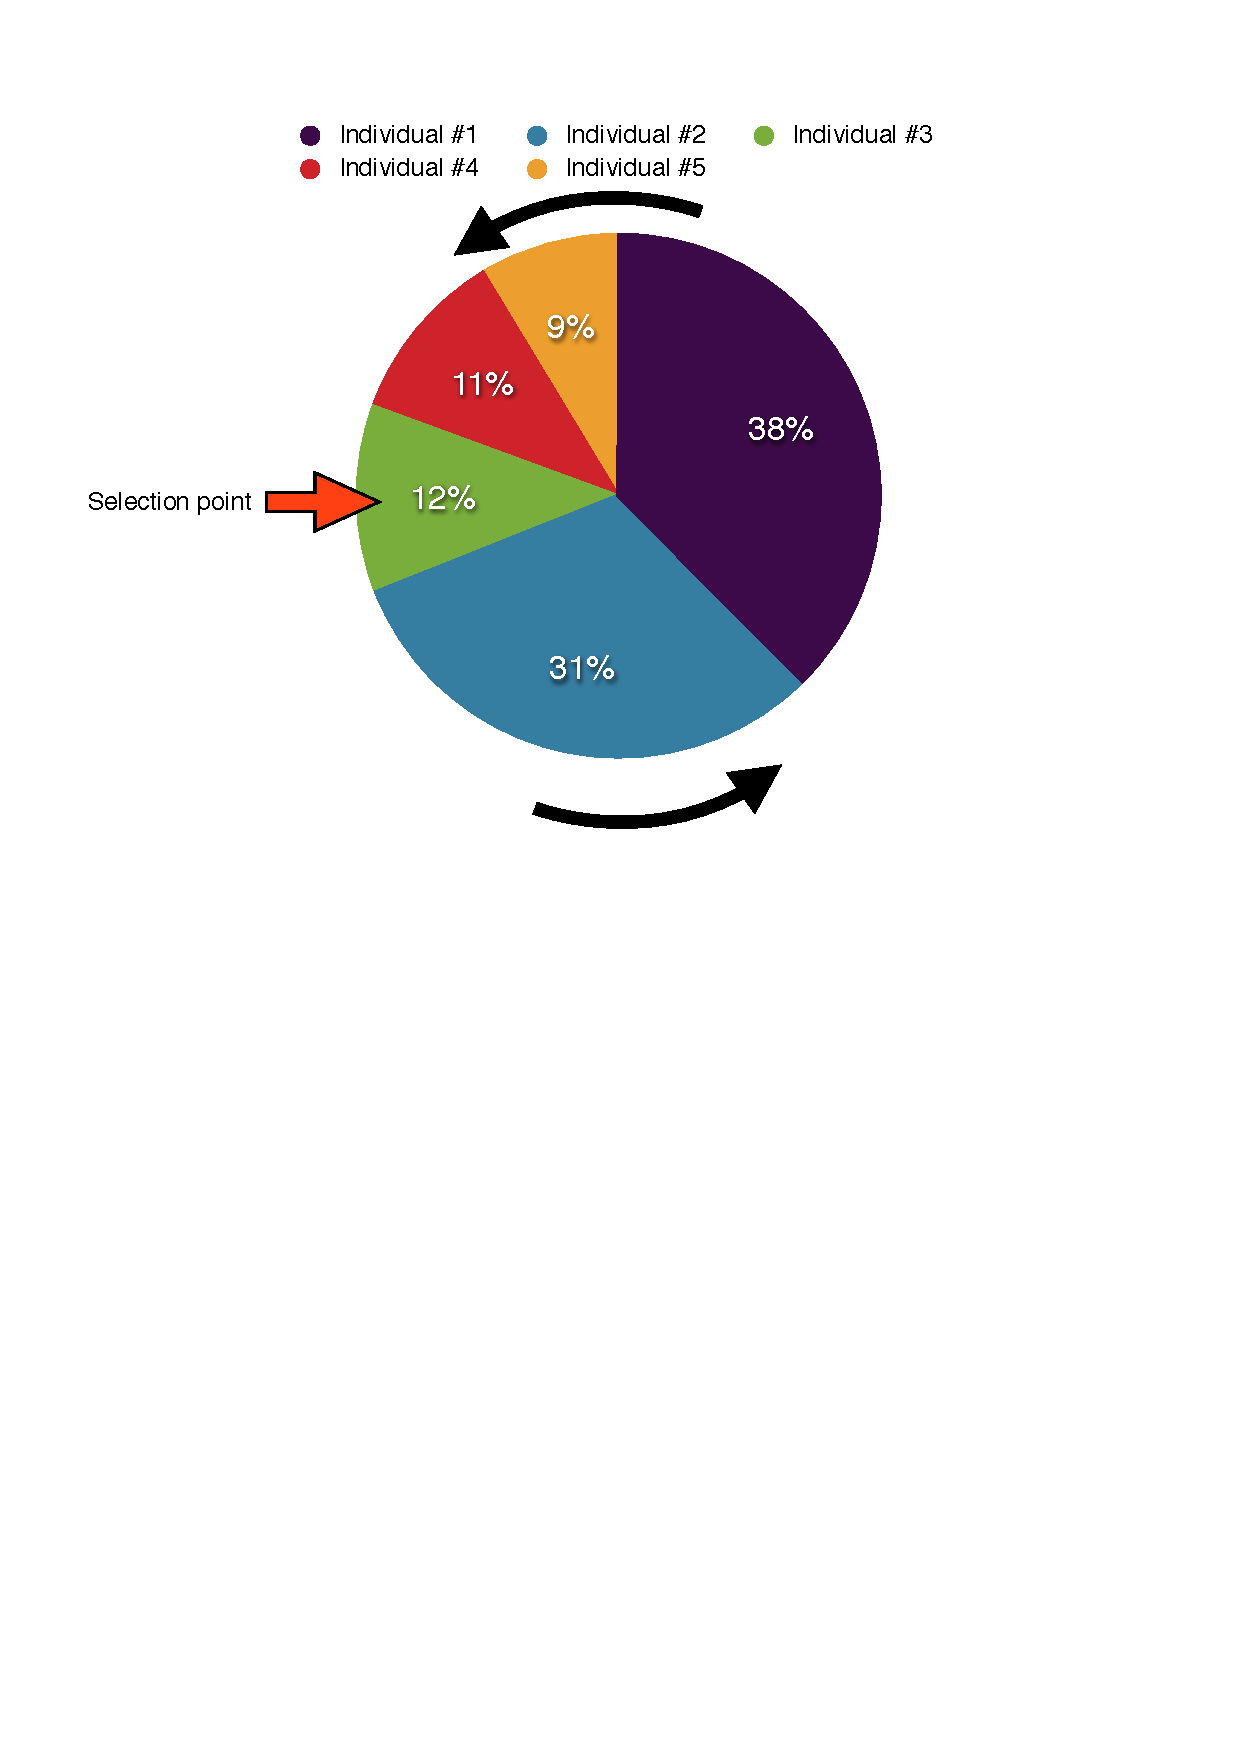
\includegraphics[width=0.7\textwidth]{chapter_ga/plots/rws_cropped.pdf} 
   \caption{The individual fitnesses are assigned proportional fractions on the roulette wheel. The wheel is then spun and will slowly decelerate and stop at some point. Individuals with a higher fitness have a higher chance of being chosen with this method.}
   \label{fig:roulettewheel}
\end{figure}

\begin{figure}[htbp] %  figure placement: here, top, bottom, or page
   \centering
   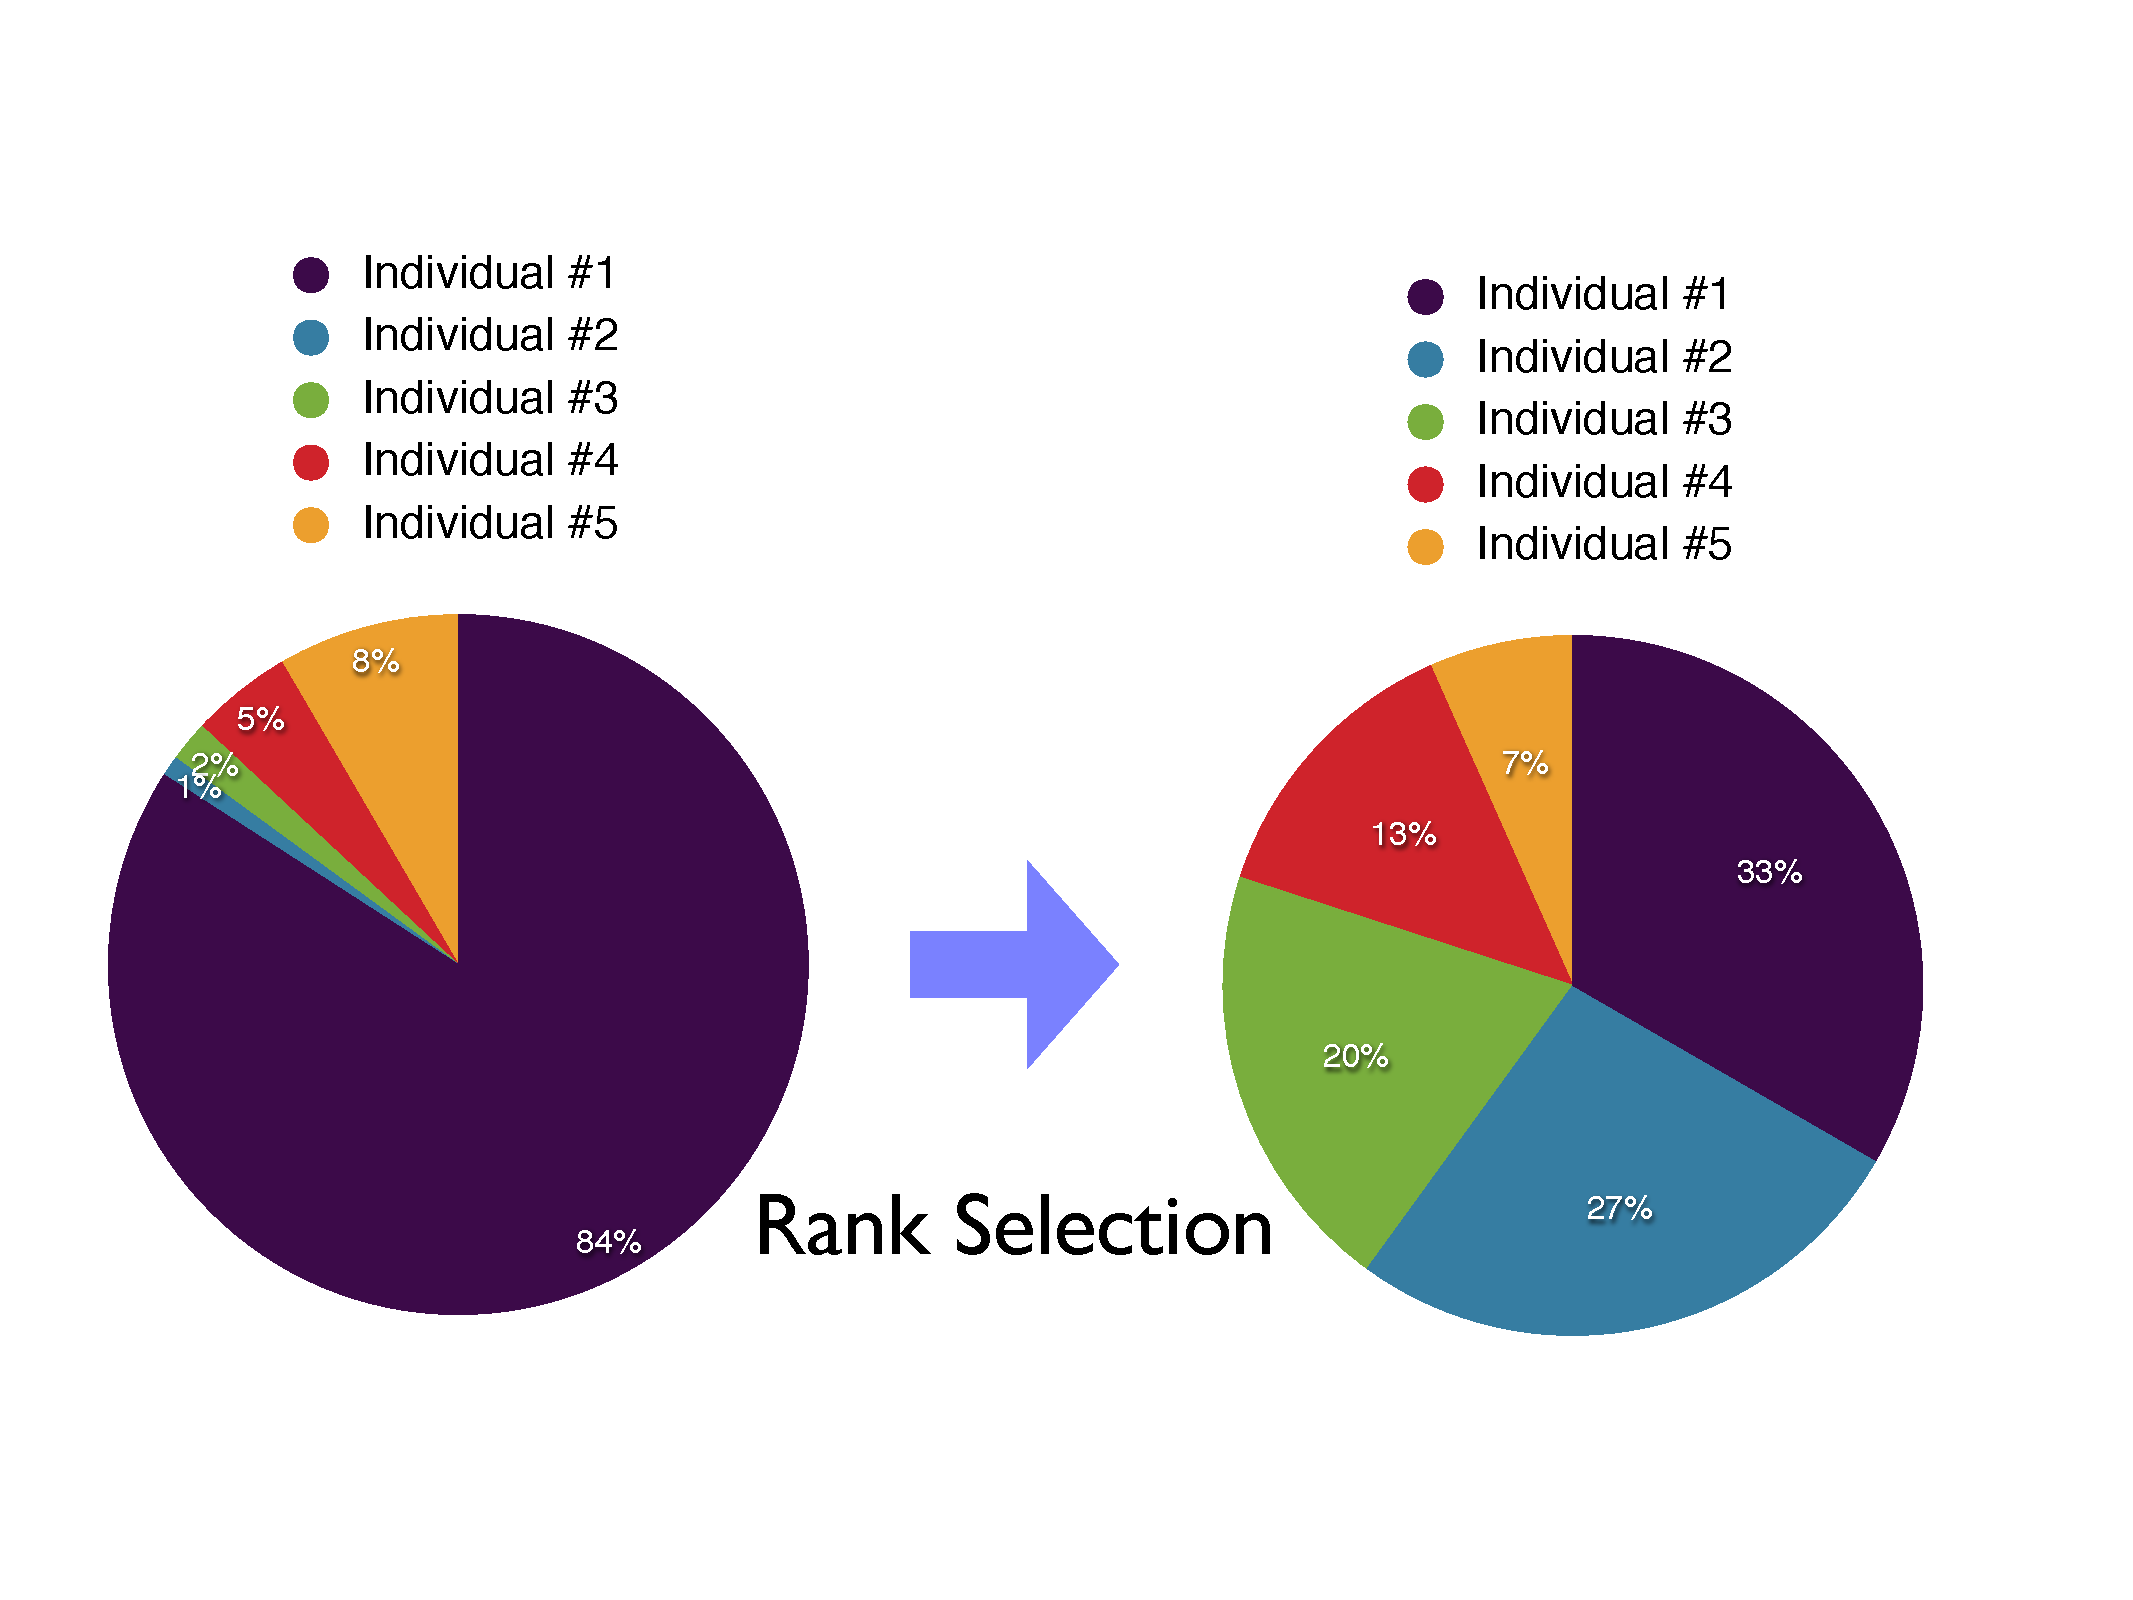
\includegraphics[width=0.7\textwidth]{chapter_ga/plots/rank_select.pdf} 
   \caption{We assign new fitness values to individuals before assigning them probabilities on the roulette wheel. The fitnesses are assigned by location in an ordered list. The least fit individual gets assigned the value 1 the fittest individual the number n, where n is the population size. This is can be viewed as a special case of fitness scaling. After the new fitnesses have been chosen we use normal roulette wheel selection to select for the mating pool in the population. }
   \label{fig:rankselection}
\end{figure}

There are multiple steps for creating a new population from the current mating population. In the previous paragraph we described how to select \glspl{individual} and place them in a mating pool. The \glspl{individual} in the mating pool are also often referred to as \glspl{parent}. Similar to the term \gls{parent} we refer to the newly created \glspl{individual} as \glspl{child}. The reader should notice that the same individual can be in the mating pool twice (unlike with biological \glspl{parent})! We create one or multiple \glspl{child} from this mating pool and place them in the next generation. The current mating pool is disbanded and a new one is formed. These steps are repeated until the new population has the same number as the old population (minus the number of individuals that advanced to the new population through \gls{elitism}). There are two main processes to create a new individual from a mating pool: \gls{crossover} and \gls{mutation}. The simplest form of a \gls{crossover} is the single-point \gls{crossover} (see Figure \ref{fig:crossover}). A random integer $r \in [1,N-1]$, where N describes the number of \glspl{gene} in a \gls{genome}, is selected. The new individual is created out of the first $r$ genes from the first parent and the last $N-r$ genes from the second parent (see Figure \ref{fig:crossover}). Now it is trivial to create a second child (using the same random number $r$) from the mating pool by just switching first and second \gls{parent}. 
Two-point \gls{crossover} is very similar to single-point crossover. In two-point \gls{crossover} Two random numbers are selected and the crossover occurs at these places. Multi-point \gls{crossover} (see Figure \ref{fig:crossover}) is essentially just an extension of two-point \gls{crossover}. In addition, there is uniform \gls{crossover} in the case that each gene is selected randomly with equal chance from either parent. Finally, arithmetic \glspl{crossover} use a function to calculate the new gene from each of the parent genes. For a value encoding this function could be the \emph{mean} function. For a binary encoding the function could be the \textit{and} operator. 
One can mix arithmetic and Multi-point  crossovers. For example we select the $r$ genes from the first parent and create the last $N-r$ genes by taking the mean of first and second parent's \glspl{gene}. After the new child or children have been created through \glspl{crossover} they are subjected to the mutation operator. There is a chance for each individual gene (often chosen to be less than 5\%) that it is altered. For bit encoding this altering is a simple bit inversions. There are many options for value encoding. For example, one can add or multiply with a random number. Once this step is complete the children are added to the new population.

\begin{figure}[htbp] %  figure placement: here, top, bottom, or page
   \centering
   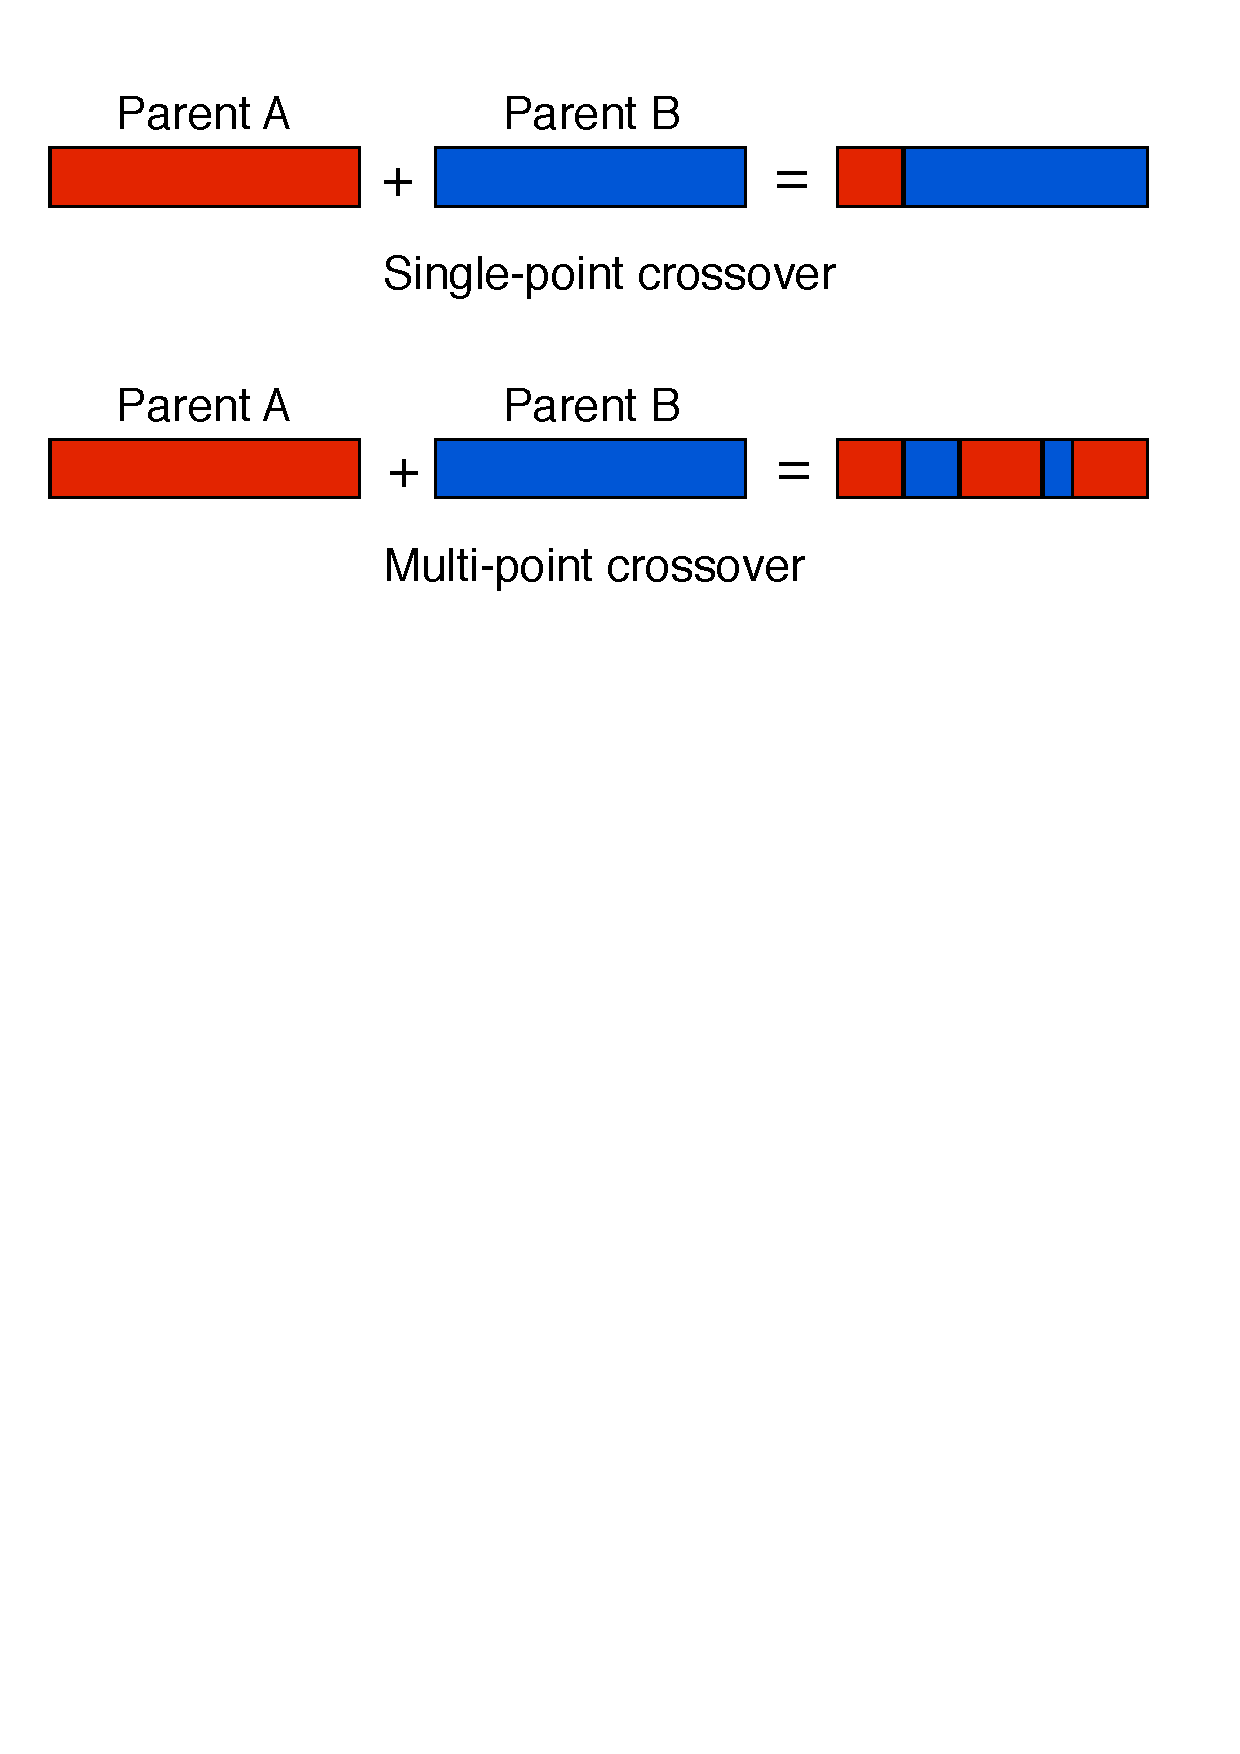
\includegraphics[width=0.7\textwidth,trim=0 18cm 0 0]{chapter_ga/plots/crossovers.pdf} 
   \caption{In the single crossover a random point in the Individual is chosen. Before this point the genes are taken from the first parent and after that the we use the genes from the second parent. Using the same random number it easily allows for the creation of two children by reversing the roles of first and second parent. The multi-point crossover employs multiple places in the genome where the crossover happens.}
   \label{fig:crossover}
\end{figure}

Once the new generation is created by \glspl{crossover} and \glspl{mutation} we start the iterative process anew. First we calculate the \gls{fitness} of all \glspl{individual}, then scale the resulting \gls{fitness}, create a mating population and select \glspl{individual} with, for example, \gls{rws}  to create children which forms the next generation. This iterative process is run until we have reached a certain number of generations or some \glspl{individual} have reached some \gls{fitness} threshold. 

\section{Convergence in Genetic Algorithms}
A key problem with many \gls{ga}-implementations is the premature convergence on a local optimum. The more complex the search space and the more interlinked the parameters are, the more likely it is that traditional search routines will fail. \glspl{ga} are inherently better at bypassing local optima but are in no way immune to this problem. A feature that separates \glspl{ga} from traditional optimization algorithms is that they will never fully converge. The algorithm will get close to the optimum but due to continued mutation of the individuals the \gls{ga} will in most cases not reach an optimal value. To alleviate this problem some authors suggest switching to a different algorithm when close to the optimum solution, whereas others suggest changing the mutation rate over time \citep[see][and references therein]{citeulike:344183}.

one of the unsolved problems is determining a mathematical description for the \glspl{ga} convergence. The predominate schemata theory explains only a subset of the intrinsic complexity of \glspl{ga}.

\section{Genetic Algorithm Theory}

The schemata theory first described by \cite{holland1975} is one of the accepted theoretical interpretations of \glspl{ga}. There is some criticism and it is known that this theory only explains part of the complexity that are inherent to \glspl{ga} \citep[see ][ and references therein]{Whitley94agenetic}. We will describe the basic concepts of schemata using an example in binary encoding \citep[notation adapted from ][]{citeulike:125978}. A schemata or similarity template is formed by adding an extra letter to the binary alphabet denoted by $*$. Using the ternary alphabet ${0, 1, *}$ we can now describe a pattern matching schemata were the $*$ symbol can be thought of as \textit{don't care}-symbol. The schemata ${0, 1, 0, *}$ for example, matches both the string ${0, 1, 0, 0}$ and ${0, 1, 0, 1}$. The order of a schemata is defined as how many places are not filled by the $*$-symbol. For example, the given example is a third order schemata. Schematas provide a powerful way to describe similarities in a set of \glspl{individual}. 
A whole population with many \glspl{individual} therefore samples a range of different schematas . Essentially low-order and above-average schemata receive exponentially increasing trials in subsequent generations of a \gls{ga}. \citet{Michalewicz:1994:GAD:184675} describe the workings of a \gls{ga} in the following way: ``A genetic algorithm seeks near optimal performance through the juxtaposition of low-order, high-performance schemata, called building blocks''.
This schemata theory is the standard explanation for \glspl{ga}, there are however some examples that violate the implications that stem from this schemata theory \citep[see chapter 3 of][for some examples]{Michalewicz:1994:GAD:184675}.

\section{A Simple Example}
We will illustrate the use of a \gls{ga} on a simple astrophysical problem. The task at hand is to fit an observed spectrum with a synthetic spectrum. The input parameters for this synthetic spectrum are \gls{teff}, \gls{logg}, \gls{feh}, $\alpha$-enhancement, \vrad and \vrot. The simplest genetic representation of this is the vector $\vec{x} = (\gls{teff}, \gls{logg}, \gls{feh}, \alpha, \vrad, \vrot)$. $\vec{x}$ is the \textit{genotype} of the individual. The resulting synthetic spectrum is the \textit{phenotype}. 

For this relatively small number of genes a population size of 75 should suffice. The first step is drawing an initial population. We will draw uniformly randomly from the search space: $\gls{teff} \in [2000, 9000]$, $\gls{logg} \in [0, 5]$, $\gls{feh} \in [-5,1]$, $\alpha \in [0,0.4]$, $\vrad \in [-100, 100]$ and $\vrot \in [0,200]$. We compute the synthetic spectrum for each individual. The fitness of each individual is the inverse of the root-mean-square of the residuals between the observed and the synthetic spectrum. 
In the select step we will first advance 10 \% of the fittest individuals to the next population unaltered (\textit{elitism}). For the next population to be complete we need $75 - 8 = 67$ individuals which are created through mating. We select two individuals through \gls{rws} and place them in the mating pool. A single crossover point is randomly selected and the child is created. Before being placed in the new population the mutation operator is applied but has a very small chance to mutate any of the child's genes (in this case we choose 2\%).
This mating step (see Figure \ref{fig:example_mating}) is repeated 67 times. The new population now consists of the 8 fittest individuals of the old population and 67 new individuals created by mating. We will then start again to compute the synthetic spectrum and the resulting fitness for each individual of the new population. This loop is continued until one individual or a whole population has reached a predefined convergence criterium.

\section{Conclusion}

\glspl{ga} with their inherently parallel nature are very useful in the increasingly parallel computing. They are relatively easy to implement and can be used for a variety of problems. In many applications \gls{ga} quickly deliver impressive results, but require a lot of time for fine-tuning to be able to sufficiently handle the problem. \glspl{ga} also offer a plethora for each of the individual steps (encoding type, selection type, etc.), which can confuse users that are not very familiar with the consequence for each choice. To alleviate this problem in our work we have sought the help of experts in \glspl{ga} and hope to find the best set of options for our \gls{ga}. 
In summary, although there are some drawbacks (no guaranteed convergence, many choices for implementation, etc.) we find that we progressed much quicker with \glspl{ga} than with other algorithms. 


